




\documentclass[a4paper]{article}

\usepackage[english]{babel}
\usepackage[utf8]{inputenc}
\usepackage{amsthm} 
\usepackage{graphicx}
\usepackage[colorinlistoftodos]{todonotes}
\usepackage{mathtools}
\usepackage{multirow}
\usepackage{tikz}
\usepackage{qtree}
\usepackage{tikz-qtree}
\usepackage[document]{ragged2e}
\usepackage{easylist}
\usepackage{amsfonts}
\usepackage{changepage}
\usepackage{fancybox}
\title{Material dialogues for Belief Revision}
\date{}
\usepackage {mathtools}
\usepackage{lipsum}
\usepackage{easylist}
\usepackage{changepage}
\usepackage{multirow}
\usepackage{multicol}

\begin{document}
\section{Examples of Pebblings}
\subsection{}
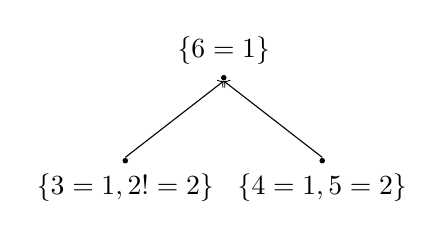
\begin{tikzpicture} 
\tikzstyle{mydot} = [circle, minimum width = 2 pt, fill, inner sep = 0 pt]  
\tikzset{every tree node/.style={mydot}, edge from parent/.append style={<-}} 
\Tree [ .\node [ mydot, label = above: {$\{6=1\}$} ] {} ;
 [.\node [ mydot, label = below: {$\{3=1, 2!=2\}$}  ] {}; ]  [.\node [ mydot, label = below:
{$\{4=1, 5=2\}$}  ] {}; ] ]

\end{tikzpicture}
\vskip 0,2 cm

This is a pebbling graph with 3 nodes. 
\vskip 0,2 cm
$Dom(6)=dom(5)=dom(4)=dom(3)=dom(2)=\{1,2\}$
\vskip 0,2 cm
Pebbling of this graph would be an I s.t.: 
\newline
$I= \{2=1, 1=1,3=1, 4=1, 5=2,6=1\}$
\newline
or an I s.t.
\vskip 0,2 cm
$I = \{2=2, 1=1, 3=2, 4=1, 5=1, 6=2\}$

\subsection{}
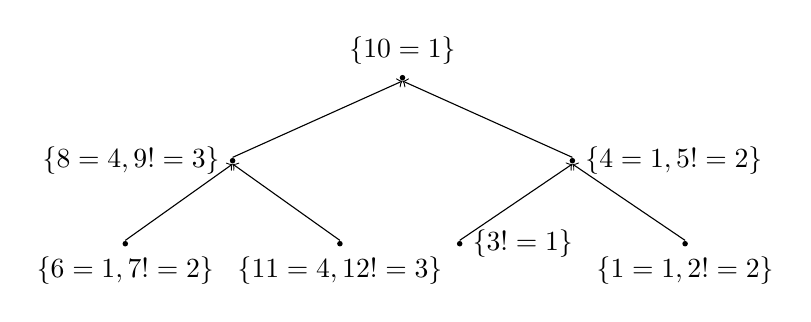
\begin{tikzpicture} 
\tikzstyle{mydot} = [circle, minimum width = 2 pt, fill, inner sep = 0 pt]  
\tikzset{every tree node/.style={mydot}, edge from parent/.append style={<-}} 
\Tree [ .\node [ mydot, label = above: {$\{10=1\}$} ] {} ;
 [.\node [ mydot, label = left: {$\{8=4, 9!=3\}$}  ] {};  [ .\node [ mydot, label = below:
{$\{6=1,7!=2\}$}  ] {};  ]   [ .\node [ mydot, label = below: {$\{11=4, 12!=3\}$}  ] {};   ]      ]
[.\node [ mydot, label = right: {$\{4=1, 5!=2\}$}  ] {}; [ .\node [
mydot, label = right: {$\{3!=1 \}$}  ] {}; ] [ .\node [ mydot, label = below: {$\{1=1, 2!=2 \}$}  ] {}; ]  ] ]
 
\end{tikzpicture}
\vskip 0,2 cm
This is a pebbling graph with 6 nodes. 
\vskip 0,2 cm
$dom(1)=dom(2)=dom(3)=dom(4)=dom(5)=dom(6)=dom(7)=dom(10)=\{1,2\}$,
\newline
$dom(8)=dom(9)=\{3,4\}$
\vskip 0,2 cm
Pebbling of this graph would be an I s.t.: 
\newline
$I= \{6=1, 12=1,3=2, 1=1, 2=1,5=1, 9=2, 10=1\}$
\newline
or an I s.t.
\vskip 0,2 cm
$I = \{1=1,2=1,3=1,4=1,5=1,6=1,7=1,11=2,12=3,8=3,9=3,10=3\}$
\vskip 0,3 cm
 Here is no illustration for pebbling problem here.
\end{document}



